\documentclass[border=5pt]{standalone}
\usepackage{amsmath,amssymb,mathtools}

\usepackage{pgfplots}
\pgfplotsset{compat=1.11}

\begin{document}
	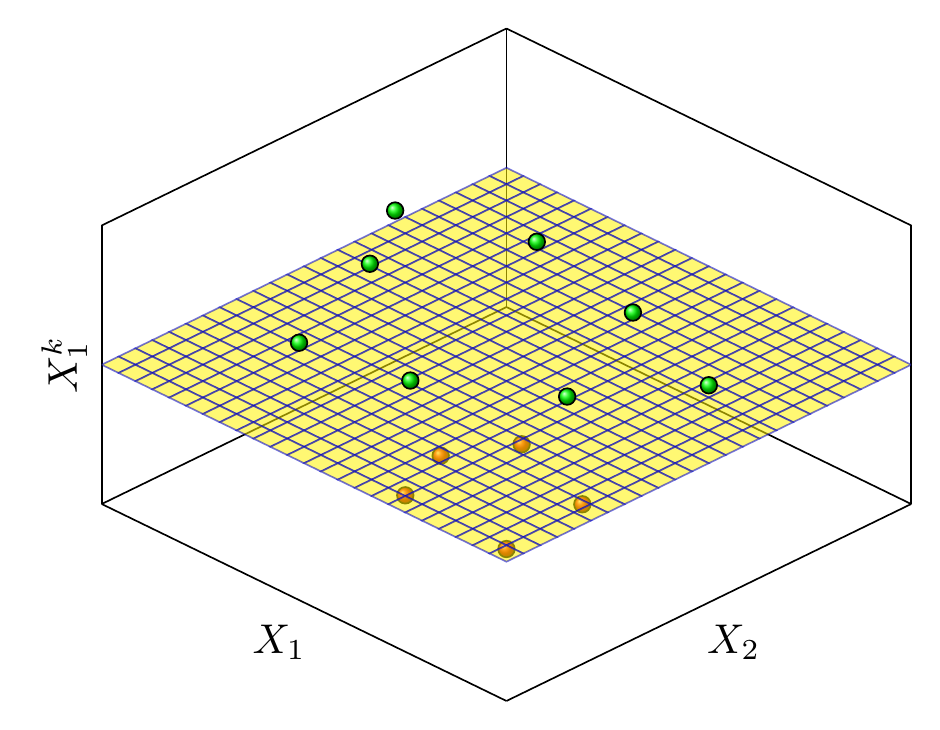
\begin{tikzpicture}[scale=1.5]
		\begin{axis}[
			view={45}{45}, % Adjust the viewing angle
			zmin=0, zmax=5,
			xmin=1, xmax=9,
			ymin=1, ymax=9,
			xlabel=$X_1$,
			ylabel=$X_2$,
			zlabel=$X_1^k$,
			xmajorticks=false,
			ymajorticks=false,
			zmajorticks=false
			]
			
			
			% Green points -------------------------------------
			\foreach \coord in {
				(5,   3,   1.04),
				(4.5, 4.2, 1   ),
				(5,   5.3, 0.94),
				(7,   3,   0.96),
				(7,   4.5, 1.1 )
			}{
				\edef\greenpoint{\noexpand\shadedraw[shading=ball, ball color=red] \coord circle (\pgfplotmarksize);}
				\greenpoint
			}
			
			
			% Yellow plane -------------------------------------
			\addplot3[surf, domain=1:9, y domain=1:9, fill=yellow, opacity=0.55] {2.5};
			
			
			% Red points ---------------------------------------
			\addplot3[only marks, mark = ball, ball color = green]
			coordinates {
				(8, 3.2, 4.05) (4.5, 6.1, 4) (9,   5,   3.9 ) (7,   5.5, 4.1)
				(6, 2.1, 3.94) (4.2, 1.7, 4) (3.5, 3.8, 4.18) (2.5, 5.3, 4.03)
			};
			
			
		\end{axis}
	\end{tikzpicture}
\end{document}